\documentclass[runningheads]{llncs}
\usepackage[T5]{fontenc}
\usepackage[utf8]{inputenc}
\usepackage{amsmath}
\usepackage{amssymb}
\usepackage{booktabs}
\usepackage{multirow}
\usepackage{url}
\usepackage{graphicx}
\usepackage{xcolor}
\usepackage{enumitem}
\usepackage{array}
\usepackage{tabularx}
\usepackage{hyperref}
\usepackage{tikz}
\usetikzlibrary{arrows.meta,positioning,fit,backgrounds}
\renewcommand{\arraystretch}{1.12}

\title{Multi-Task PhoBERT for Vietnamese Spam-Review Type Classification:
Reproduction, Controlled Improvement, and Product-Disjoint Robustness}
\titlerunning{Multi-Task PhoBERT for Vietnamese Spam-Review Classification}

\author{Phan Bá Song Toàn\inst{1} \and
Trịnh Minh Bảo Trân\inst{1} \and
Trần Quang Long\inst{1}}
\authorrunning{P. B. S. Toàn et al.}
\institute{TMG301 Text Mining, Vietnam}

\begin{document}
\maketitle

\begin{abstract}
Vietnamese e-commerce review platforms contain both legitimate reviews and several types of spam reviews. This paper presents a controlled empirical study of Vietnamese spam-review classification using the ViSpamReviews v2 dataset and PhoBERT. First, we reproduce a single-task PhoBERT baseline under a fixed training protocol. Second, we propose a lightweight multi-task architecture with a shared PhoBERT encoder and two classification heads: a binary spam detector and a three-class spam-type classifier. Third, we evaluate generalization under a product-disjoint split, in which reviews from the same product are not shared across train, development, and test sets. On the official released split, the reproduced PhoBERT baseline obtains 76.69\% Macro-F1 on the four-class task, while the multi-task model obtains 77.42\%. On the more demanding product-disjoint split, the multi-task model obtains 90.96\% accuracy and 76.73\% Macro-F1. The results show a small improvement from multi-task supervision under the locked protocol and a limited robustness gap between random and product-disjoint evaluation. We also report unsuccessful alternatives, including weighted loss and rule augmentation, to make the experimental conclusions transparent.
\end{abstract}

\keywords{Vietnamese NLP \and spam review detection \and PhoBERT \and multi-task learning \and e-commerce \and robustness \and product-disjoint evaluation}

\section{Introduction}
Online reviews influence product discovery and purchasing decisions, but review platforms also contain content that is repetitive, promotional, strategically manipulated, or otherwise unreliable. Vietnamese spam-review detection is challenging because user-generated text contains spelling variation, abbreviations, code-switching, short comments, and product-specific language.

The paper by Tran et al.\cite{originalpaper} studies spam-review detection on Vietnamese e-commerce websites and integrates review metadata with neural text classifiers. It reports a four-class task and a binary task, and evaluates TextCNN, BiLSTM, BiGRU, PhoBERT, and BERT4News. Its results provide a useful reference point, but a random review split can overestimate generalization when reviews from the same product occur in both training and test data.

The gap addressed here is methodological rather than purely architectural: the published setting does not isolate the effect of hierarchical supervision or test whether the model generalizes to products unseen during training. This work has three objectives:
\begin{enumerate}[leftmargin=*]
    \item establish a reproducible PhoBERT baseline using the publicly released ViSpamReviews v2 split;
    \item test whether joint binary spam detection and spam-type classification improves the four-class task; and
    \item measure robustness when products are held out from training.
\end{enumerate}

The contribution is therefore an auditable evaluation rather than an unsupported claim of state-of-the-art performance. All primary metrics, configurations, logs, checkpoints, and reports are retained as experiment artefacts.

\section{Background and Related Work}
\subsection{Vietnamese spam-review classification}
The original study defines two related tasks. Task 1 is binary classification between non-spam and spam reviews. Task 2 is four-class classification: non-spam plus three spam types. In the original experiments, review text is combined with product category and description in several metadata configurations. The study reports that PhoBERT is the strongest text-oriented model among the evaluated baselines, while metadata integration can improve performance in selected settings\cite{originalpaper}.

\subsection{PhoBERT}
PhoBERT is a RoBERTa-style pretrained language model designed for Vietnamese text\cite{phobert}. It uses subword tokenization and contextual self-attention, following the transformer pretraining paradigm\cite{bert}. In this study, the pretrained encoder is fine-tuned rather than trained from scratch. This is appropriate for the course and task because the model learns task-specific decision boundaries from labeled reviews while retaining Vietnamese linguistic knowledge from pretraining.

\subsection{Multi-task learning}
Multi-task learning trains related objectives with a shared representation\cite{multitask}. Here, the encoder is shared by a binary head and a spam-type head. The binary head predicts whether a review is spam, while the type head predicts one of the three spam types for spam examples. The total loss is:
\begin{equation}
\mathcal{L}=\mathcal{L}_{bin}+\mathbb{I}(y_{bin}=1)\mathcal{L}_{type},
\end{equation}
where the type loss is calculated only for spam examples. At inference time, a binary non-spam prediction becomes class 0; otherwise, the type-head prediction is mapped to classes 1--3.

\subsection{Research positioning}
The proposed contribution is a controlled extension of the published text-classification setting. It does not claim a new pretrained language model. Instead, it contributes (i) a hierarchical multi-task objective aligned with the dataset labels, (ii) a product-disjoint robustness protocol, and (iii) an auditable comparison of interventions that did and did not improve Macro-F1.

\section{Dataset and Data Audit}
\subsection{Dataset}
The experiments use the publicly released \texttt{sonlam1102/vispamdetection2} version of ViSpamReviews v2. The release contains the review comment, rating, product category, product name, product description, sales and review-count metadata, a binary label, and a four-class spam label. The released split contains 14,306 training examples, 1,590 validation examples, and 3,974 test examples.

The paper reports slightly different counts (14,284/1,589/3,963). Therefore, the reproduction in this paper is explicitly an approximate reproduction of the published experiment on the public release, not a claim that the unavailable internal snapshot was recreated exactly.

\subsection{Label distribution}
On the official test split, the four-class supports are 2,914, 54, 310, and 696 for classes 0, 1, 2, and 3, respectively. The severe imbalance makes Macro-F1 more informative than accuracy alone.

\subsection{Product leakage audit}
To test whether random splitting may expose product-specific information, product groups were normalized from product name, category, and description. The audit found overlapping normalized product groups between train and dev (996), train and test (1,456), and dev and test (921). These overlaps motivate a secondary product-disjoint evaluation.

For that evaluation, GroupShuffleSplit was applied to the normalized product key. The resulting split contains 13,985 train, 1,947 development, and 3,938 test examples. Its test supports are 2,961, 49, 284, and 644 for classes 0--3.

\section{Experimental Method}
\subsection{Reproduction protocol}
The primary reproduction uses \texttt{vinai/phobert-base-v2}, PhoBERT tokenization, maximum sequence length 100, batch size 16, AdamW optimization, encoder learning rate $10^{-5}$, classification-head learning rate $5\times10^{-5}$, cross-entropy loss, seed 42, and early stopping based on development Macro-F1. The same protocol is used for the single-task and multi-task primary comparisons. No class weighting or logit adjustment is used in the reproduction baseline.

\subsection{Baseline}
The baseline is a standard PhoBERT sequence-classification model. The pooled first-token representation is passed to a linear classification head. For Task 2, the head predicts four classes directly. This model is intentionally simple: it isolates the effect of the proposed multi-task supervision from changes in preprocessing, dataset, or backbone.

\subsection{Proposed model}
The proposed model uses one shared PhoBERT encoder followed by two dropout-linear heads. The binary head has two outputs and the type head has three outputs. During training, the type head is supervised only on spam reviews. During prediction, the binary decision gates the type prediction. This design introduces a hierarchy aligned with the label structure without changing the pretrained encoder architecture.

\begin{figure}[t]
\centering
\resizebox{0.98\linewidth}{!}{%
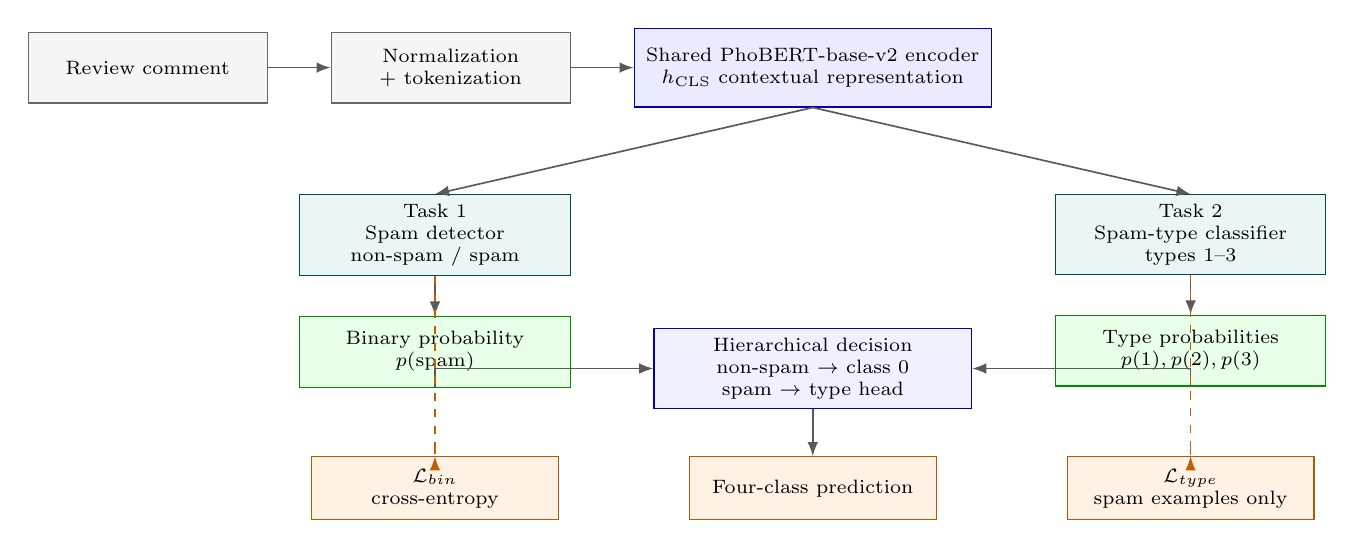
\begin{tikzpicture}[
  font=\scriptsize,
  >=Latex,
  node distance=6mm and 8mm,
  input/.style={draw=black!60, fill=gray!8, align=center,
    minimum height=9mm, text width=28mm},
  encoder/.style={draw=blue!65!black, fill=blue!8, align=center,
    minimum height=10mm, text width=43mm},
  head/.style={draw=teal!60!black, fill=teal!8, align=center,
    minimum height=10mm, text width=32mm},
  output/.style={draw=green!55!black, fill=green!9, align=center,
    minimum height=9mm, text width=32mm},
  gate/.style={draw=blue!65!black, fill=blue!6, align=center,
    minimum height=10mm, text width=38mm},
  loss/.style={draw=orange!70!black, fill=orange!10, align=center,
    minimum height=8mm, text width=29mm},
  arrow/.style={-{Latex[length=1.8mm]}, semithick, draw=black!65},
  objective/.style={-{Latex[length=1.8mm]}, semithick, dashed, draw=orange!75!black}
]
\node[input] (review) {Review comment};
\node[input, right=of review] (token) {Normalization\\+ tokenization};
\node[encoder, right=of token] (encoder) {Shared PhoBERT-base-v2 encoder\\$h_{\mathrm{CLS}}$ contextual representation};
\node[head, below left=11mm and 8mm of encoder] (binary) {Task 1\\Spam detector\\non-spam / spam};
\node[head, below right=11mm and 8mm of encoder] (type) {Task 2\\Spam-type classifier\\types 1--3};
\node[output, below=5mm of binary] (binout) {Binary probability\\$p(\mathrm{spam})$};
\node[output, below=5mm of type] (typeout) {Type probabilities\\$p(1),p(2),p(3)$};
\node[gate, below=28mm of encoder] (gate) {Hierarchical decision\\non-spam $\rightarrow$ class 0\\spam $\rightarrow$ type head};
\node[loss, below=6mm of gate] (final) {Four-class prediction};
\node[loss, below left=6mm and 12mm of gate] (binloss) {$\mathcal{L}_{bin}$\\cross-entropy};
\node[loss, below right=6mm and 12mm of gate] (typeloss) {$\mathcal{L}_{type}$\\spam examples only};
\draw[arrow] (review) -- (token);
\draw[arrow] (token) -- (encoder);
\draw[arrow] (encoder.south) -- (binary.north);
\draw[arrow] (encoder.south) -- (type.north);
\draw[arrow] (binary) -- (binout);
\draw[arrow] (type) -- (typeout);
\draw[arrow] (binout.south) |- (gate.west);
\draw[arrow] (typeout.south) |- (gate.east);
\draw[arrow] (gate) -- (final);
\draw[objective] (binary.south) |- (binloss.north);
\draw[objective] (type.south) |- (typeloss.north);
\end{tikzpicture}
}%
\caption{Overview of the proposed hierarchical multi-task PhoBERT model.}
\label{fig:architecture}
\end{figure}

\subsection{Controlled alternatives}
The following variants were tested during development: class-weighted loss, focal loss, class-balanced loss, logit adjustment, threshold tuning, raw metadata fusion, category-only input, description-only input, separate fusion, gated fusion, attentive pooling, and rule-augmented multi-task learning. These experiments are treated as exploratory ablations. They are reported to avoid selective reporting, but only the locked baseline and multi-task comparison are used for the main claim.

\subsection{Evaluation metrics}
Accuracy is reported for comparability with prior work. Macro-F1 is the primary metric because it gives equal importance to rare spam classes:
\begin{equation}
F1_{macro}=\frac{1}{K}\sum_{k=1}^{K}F1_k.
\end{equation}
Per-class precision, recall, and F1 are also reported. Product-disjoint performance is used as a robustness measure, not as a replacement for the official split.

\section{Results}
\subsection{Published reference and reproduction}
Table~\ref{tab:reference} separates published numbers from our runs. The published results come from the original paper and use its reported dataset version. Our reproduction uses the public release and must therefore be interpreted within that limitation.

\begin{table}[t]
\caption{Published reference and our PhoBERT reproduction.}
\label{tab:reference}
\centering
\small
\begin{tabularx}{0.95\linewidth}{Xcc}
\toprule
Setting & Accuracy & Macro-F1 \\
\midrule
Published PhoBERT Task 1 & 89.23\% & 85.58\% \\
Published PhoBERT Task 2 & 87.79\% & 71.56\% \\
Our reproduction Task 1 & 91.55\% & 89.04\% \\
Our reproduction Task 2 & 91.37\% & 76.69\% \\
\bottomrule
\end{tabularx}
\end{table}

The difference between the published and reproduced numbers is not interpreted as a direct improvement over the paper because the public and reported dataset snapshots differ. The reproduction establishes an internal baseline for controlled experiments.

\subsection{Main comparison}
\begin{table}[t]
\caption{Main comparison on the official released split.}
\label{tab:main}
\centering
\small
\begin{tabularx}{0.95\linewidth}{Xlcc}
\toprule
Model & Task & Accuracy & Macro-F1 \\
\midrule
PhoBERT reproduction & Task 2 & 91.37\% & 76.69\% \\
Multi-task PhoBERT & Task 2 & \textbf{91.12\%} & \textbf{77.42\%} \\
\midrule
Multi-task binary head & Task 1 & 91.95\% & 89.51\% \\
\bottomrule
\end{tabularx}
\end{table}

The multi-task model improves Task 2 Macro-F1 by 0.73 percentage points relative to the reproduction baseline, although its accuracy is slightly lower. This is the preferred trade-off because Macro-F1 better reflects performance on rare classes.

\subsection{Product-disjoint robustness}
\begin{table}[t]
\caption{Generalization to unseen products.}
\label{tab:product}
\centering
\small
\begin{tabularx}{0.95\linewidth}{Xcc}
\toprule
Evaluation & Accuracy & Macro-F1 \\
\midrule
Random split, multi-task & 91.12\% & 77.42\% \\
Product-disjoint, multi-task & 90.96\% & 76.73\% \\
Difference & -0.16 pp & -0.69 pp \\
\bottomrule
\end{tabularx}
\end{table}

The small decrease indicates that the model retains most of its performance when product overlap is removed. This result is more informative than a random-split score alone because it tests whether the model relies excessively on product-specific wording.

\subsection{Exploratory ablations}
\begin{table}[t]
\caption{Selected exploratory experiments on Task 2.}
\label{tab:ablations}
\centering
\small
\begin{tabularx}{0.95\linewidth}{Xcc}
\toprule
Variant & Accuracy & Macro-F1 \\
\midrule
Multi-task PhoBERT & 91.12\% & 77.42\% \\
Rule-augmented multi-task & 91.02\% & 75.12\% \\
Weighted type loss & 90.26\% & 71.11\% \\
Category-only control & 90.46\% & 75.23\% \\
Description-only control & 88.78\% & 74.50\% \\
Separate fusion control & 88.42\% & 74.45\% \\
\bottomrule
\end{tabularx}
\end{table}

The exploratory results do not support adding class weights, the tested rule features, or the evaluated fusion variants to the main model. In particular, the weighted type loss reduces Macro-F1, suggesting that naive reweighting may overcompensate for the minority classes. These results are useful negative findings, but they should be rerun under the final locked protocol before being presented as strict causal ablations.

\subsection{Per-class analysis}
On the product-disjoint test set, the multi-task model obtains F1 scores of 0.94, 0.56, 0.67, and 0.89 for classes 0--3, respectively. Class 1 remains the hardest class because it has only 49 test examples. The model has high performance on the majority non-spam class and class 3, but recall for class 1 is only 0.49. This confirms that aggregate accuracy alone would hide the main weakness.

\begin{table}[!b]
\caption{Per-class product-disjoint test results.}
\label{tab:perclass}
\centering
\small
\begin{tabularx}{0.95\linewidth}{X c c c c}
\toprule
Class & Support & Precision & Recall & F1 \\
\midrule
0 & 2,961 & 0.94 & 0.95 & 0.94 \\
1 & 49 & 0.67 & 0.49 & 0.56 \\
2 & 284 & 0.61 & 0.75 & 0.67 \\
3 & 644 & 0.94 & 0.84 & 0.89 \\
\midrule
Macro average & 3,938 & 0.79 & 0.76 & 0.77 \\
\bottomrule
\end{tabularx}
\end{table}

\section{Discussion}
The main result is not that the proposed model universally beats the original paper. Instead, the controlled study shows three defensible findings. First, the public dataset and published dataset counts differ, so claims must distinguish reproduction from direct comparison. Second, multi-task supervision provides a small Macro-F1 gain over a matched PhoBERT baseline. Third, product-disjoint evaluation produces only a modest drop, suggesting reasonable cross-product generalization.

The experiments also demonstrate why proposed improvements should be evidence-driven. More complex fusion, rule augmentation, and naive class weighting did not improve the main metric. A method that is simpler but stable under a stricter split is preferable to a method that produces a higher accuracy through uncontrolled changes.

\section{Limitations}
The study has several limitations. The exact internal dataset snapshot used by the original paper is unavailable, preventing exact reproduction. Most experiments use a single seed, so confidence intervals and statistical significance are not yet established. The product grouping key is constructed from available metadata and may merge or separate products imperfectly. The minority classes remain small, especially class 1, which makes its F1 estimate unstable. Finally, the current proposed architecture changes the supervision objective but does not introduce a new pretrained backbone.

\section{Future Work}
The next experiments should use three to five seeds, report mean and standard deviation, lock one configuration for all ablations, and perform systematic error analysis. Future architectural extensions may include calibrated hierarchical prediction, contrastive learning across product groups, and explicit handling of duplicated or near-duplicated reviews. Each extension must be compared against the same reproduced baseline.

\section{Reproducibility Statement}
All primary experiments use seed 42 and retain their configuration, training log, best checkpoint, final metrics, and classification report. The public dataset identifier, model checkpoint, split construction, maximum sequence length, optimizer, learning rates, batch size, and early-stopping rule are specified in this paper. The main comparison is restricted to the locked PhoBERT reproduction and the multi-task model; exploratory alternatives are not used to replace the primary baseline.

\section{Conclusion}
This paper presented a reproducible and controlled study of Vietnamese spam-review type classification with PhoBERT. A shared-encoder multi-task model improved Task 2 Macro-F1 from 76.69\% to 77.42\% on the public official split and achieved 76.73\% Macro-F1 when evaluated on unseen products. The results support multi-task supervision as a modest, practical improvement, while the product-disjoint experiment provides evidence that the result is not solely caused by product overlap. The study deliberately avoids claiming an absolute improvement over the original publication because the released and reported dataset versions are not identical. The resulting evaluation is therefore more transparent, reproducible, and suitable as a foundation for further research.

\begin{thebibliography}{00}
\bibitem{originalpaper}
Co Van Dinh and Son T. Luu, ``Metadata Integration for Spam Reviews Detection on Vietnamese E-commerce Websites,'' arXiv:2405.13292, 2024. [Online]. Available: \url{https://arxiv.org/abs/2405.13292}. Published in the International Journal of Asian Language Processing.

\bibitem{phobert}
D. Q. Nguyen and A. T. Nguyen, ``PhoBERT: Pre-trained language models for Vietnamese,'' in \emph{Findings of EMNLP}, 2020, pp. 1037--1042.

\bibitem{bert}
J. Devlin, M.-W. Chang, K. Lee, and K. Toutanova, ``BERT: Pre-training of deep bidirectional transformers for language understanding,'' in \emph{Proc. NAACL-HLT}, 2019, pp. 4171--4186.

\bibitem{multitask}
R. Caruana, ``Multitask learning,'' \emph{Machine Learning}, vol. 28, pp. 41--75, 1997.
\end{thebibliography}

\end{document}
